\chapter{Policy in the AS/AD model \index{AS/AD model}
}\label{chp:pasad}
\hypertarget{asadpolicy}{}

%No extra line here.
\textbf{Tools:} Aggregate supply and demand (AS/AD) graph.

\textbf{Key Words:} Policy objectives; potential output; output gap.

\textbf{Big Ideas:}
%\vspace{-0.1in}
\begin{itemize}
    \item The objectives of monetary policy are generally thought to be (i)~stable prices and (ii)~output near its long-run equilibrium level.
\item A direct consequence is that monetary policy should respond differently to demand and supply shocks.
As a general rule, policy should resist/offset changes in output triggered by shifts in demand
and accommodate/reinforce changes triggered by shifts in supply.
    \item We can identify supply or demand shocks from whether output and prices move together or in opposite directions.
\end{itemize}

\rule{\textwidth}{1pt}

We've seen that aggregate demand
 and supply can shift on their own or,
sometimes, as a result of changes in policy,
including monetary policy.
But what policy changes are called for?
Should we always shift the aggregate demand
 curve to maintain
low inflation?\index{inflation}  High output?
Are these two objectives in conflict?
The short answer is that we should respond differently to changes in supply and demand.
A somewhat longer answer follows.


\section{Objectives of policy}

The traditional guide to economic policy is the invisible hand.
If markets work well, then we simply leave them to do their job.
If not, we may act to facilitate their operation.
In the aggregate demand\index{aggregate demand (AD)}
 and supply framework,
the idea is that the   long-run aggregate supply \index{aggregate supply (AS)!long-run aggregate supply}\index{aggregate supply (AS)}
 curve is where the uninhibited operation of markets would lead us.
In the short run, sticky wages (or other market imperfections)
may delay the adjustment, but that's
where the invisible hand ultimately would direct us.
One consequence is that there's no
compelling reason to change aggregate demand \index{aggregate demand (AD)}
to increase output beyond its long-run equilibrium value.
We might be able to do it, but it won't make us better off.
In a sense, we will have tricked people into working more than they
want, typically by reducing their real wages through unexpected inflation.\index{inflation}

The first objective of policy, then,
is to get output as near as possible to
the level associated with the long-run
aggregate supply\index{aggregate supply (AS)}
 curve AS$^*$.
This is important enough a concept that people have given it
lots of names:  potential output, full employment output, and so on.
We'll call it {\it potential output\index{potential output}\/}, with the understanding that it's
the long-run equilibrium, not an upper bound.
The {\it output gap \index{output gap}\/} is a related concept:
the difference between actual and potential output.
In practice, potential output is a little slippery,
because the   long-run aggregate supply \index{aggregate supply (AS)!long-run aggregate supply}\index{aggregate supply (AS)}
 curve isn't something we observe.
We have a variety of ways of estimating potential output,
ranging from the complex  to
the pragmatic (a smooth trend line drawn through actual output).
We give some examples (and links) at the end of the chapter.

The second objective of policy is price stability.
That's not an obvious implication of the invisible hand,
but experience has taught us that low and (especially) stable rates of
inflation\index{inflation} are associated with good macroeconomic performance.
You might ask whether we'd be better off with no inflation,
low inflation (say, two or three percent a year),
or even modest deflation (yes, there are theoretical arguments
for that).
However, experience suggests that it doesn't matter too much. Any stable target is better than
the high and variable inflation that the US and many other countries
experienced in the 1970s.


%%%%%%%%%%%%%%%%%%%%%%%%%%%%%%%%%%%%%%%%%%%%%%%%%%%%%%%%%%%%%%%%%%%%%%%%%%%%
%  Supply and demand diagram
\begin{figure}[h!]
\caption{The impact of an adverse demand shock.}
    \label{fig:asad-m}
%
\centering
\setlength{\unitlength}{0.075em}
\begin{picture}(250,200)(0,0)
%\footnotesize
\thicklines

% horizontal axis
\put(-30,0){\vector(1,0){300}}
\put(255,-16){$Y$}
\put(142,-16){$Y^*$}

% vertical axis
\put(0,-20){\vector(0,1){200}}
\put(-15,155){$P$}

% demand
\put(25,165){\line(4,-3){200}}\put(230,10){AD$'$}
\put(65,165){\line(4,-3){200}}\put(270,10){AD}

% supply
\put(25,13){\line(4,3){200}} \put(230,160){AS}
%\put(65,13){\line(4,3){200}} \put(270,160){AS$'$}
\put(146.4,0){\line(0,1){170}} \put(138,175){AS$^*$}

% equilibrium labels
\put(105,85){\footnotesize B}
\put(150,115){\footnotesize A}
%\put(138,64){\footnotesize C}
% dotted lines
%\qbezier[31]{(133,0)(133,46)(133,92)}
%\qbezier[45]{(0,92)(67,92)(133,92)}
%\qbezier[45]{(0,72)(67,72)(133,72)}

\end{picture}
\begin{minipage}{0.7\textwidth}
\vspace{0.45in}
{\footnotesize Aggregate demand\index{aggregate demand (AD)}
 AD shifts left to AD$'$, moving the short-run equilibrium from A to B.}
\end{minipage}

\end{figure}
%%%%%%%%%%%%%%%%%%%%%%%%%%%%%%%%%%%%%%%%%%%%%%%%%%%%%%%%%%%%%%%%%%%%%%%%%%%%



\section{Policy responses to supply and demand shocks}

With potential output and stable prices as our objectives,
how should policy respond to changes in aggregate supply\index{aggregate supply (AS)}
 or demand?
Curiously, the answer depends on whether we face supply shocks or demand
shocks.

How should we respond to demand shocks?
Consider a negative demand shock,
illustrated by Figure \ref{fig:asad-m}.
The long-run equilibrium is point A,
where aggregate supply\index{aggregate supply (AS)}
 AS$^*$ and aggregate demand\index{aggregate demand (AD)}
 AD cross.
Suppose that consumer pessimism shifts the aggregate demand\index{aggregate demand (AD)}
 curve to AD$'$, leaving us at point B.
What should we do?
If we do nothing, we fail on both of our objectives because output is below potential and prices have fallen.
The appropriate policy, then, is to shift the demand curve
back to AD, perhaps by expanding the money supply.

That's a general rule:  Policy should offset demand shocks.
In this case, there is no conflict between our two goals
of hitting potential output and maintaining stable prices.
The policy lesson:  We should resist or offset demand shocks.


%%%%%%%%%%%%%%%%%%%%%%%%%%%%%%%%%%%%%%%%%%%%%%%%%%%%%%%%%%%%%%%%%%%%%%%%%%%%
%  Supply and demand diagram
\begin{figure}[h!]
\caption{The impact of an increase in the price of oil.}
\label{fig:asad-oil}
%
\centering
\setlength{\unitlength}{0.075em}
\begin{picture}(250,200)(0,0)
%\footnotesize
\thicklines

% horizontal axis
\put(-30,0){\vector(1,0){300}}
\put(255,-16){$Y$}
\put(142,-16){$Y^*$}
\put(102,-16){$Y^{*\prime}$}

% vertical axis
\put(0,-20){\vector(0,1){200}}
\put(-15,155){$P$}

% demand
\put(25,165){\line(4,-3){200}}\put(230,10){AD}
%\put(65,165){\line(4,-3){200}}\put(270,10){AD$'$}

% supply
\put(65,13){\line(4,3){200}} \put(270,160){AS}
\put(25,13){\line(4,3){200}} \put(230,160){AS$'$}
\put(146.4,0){\line(0,1){170}} \put(138,175){AS$^*$}
\put(106.4,0){\line(0,1){170}} \put(98,175){AS$^{*\prime}$}

% equilibrium labels
\put(150,55){\footnotesize A}
\put(122,75){\footnotesize B}
\put(95,94){\footnotesize C}
\put(95,76){\footnotesize D}
%\put(95,54){\footnotesize D}
% dotted lines
%\qbezier[31]{(133,0)(133,46)(133,92)}
%\qbezier[45]{(0,92)(67,92)(133,92)}
%\qbezier[45]{(0,72)(67,72)(133,72)}

\end{picture}
\begin{minipage}{0.7\textwidth}
\vspace{0.45in}
{\footnotesize Aggregate supply\index{aggregate supply (AS)}
 curves shift left from AS/AS$^*$ to AS$'$/AS$^{*\prime}$,
moving the short-run equilibrium from A to B.}
\end{minipage}

\end{figure}
%%%%%%%%%%%%%%%%%%%%%%%%%%%%%%%%%%%%%%%%%%%%%%%%%%%%%%%%%%%%%%%%%%%%%%%%%%%%


How should we respond to supply shocks? \index{supply shocks}
Consider the situation depicted in Figure \ref{fig:asad-oil}:
an adverse supply shock that moves us from A to B.
Should policy try to offset the decline in output?
If we follow our logic, the answer is no;
we want to move output as close to the long-run aggregate supply \index{aggregate supply (AS)!long-run aggregate supply}\index{aggregate supply (AS)}
curve AS$^{*\prime}$ as possible.
We do this by moving the aggregate demand\index{aggregate demand (AD)}
 curve left (left!) until it intersects
both aggregate supply\index{aggregate supply (AS)}
 curves at point D.
At this point, the price level is the same as it was at A,
so we have delivered stable prices.
Output has fallen more than if we had not acted,
but that's what the invisible hand suggests.
The policy lesson:  We should acquiesce to or accommodate
supply shocks.

The basic lesson, then, is that we want to react differently to
changes in output that result from supply and demand shocks.
We should resist demand shocks and accommodate supply shocks.
The difficulty, in practice, is knowing which is which.
If we guess wrong, we can make things worse, perhaps a lot worse.

By some interpretations, the Fed made exactly that mistake in the 1970s.
With output falling and inflation rising, the Fed increased the money
supply to keep output up.
With hindsight, the OPEC oil price increase is understood to be an
adverse supply shock.
It reduced output, but there was little we could do about it.
When we increased the money supply, the consequence was that low
output was accompanied by even higher inflation\index{inflation} than before.
Having failed to understand the nature of the problem,
we gave it a name:  stagflation.


\section*{Executive summary}

\setlength{\leftmargini}{.5\oldleftmargini}
\begin{enumerate}
\item We typically think of the goals of macroeconomic
policy as keeping inflation low and output near the long-run
supply curve.

\item As a general rule, policy should resist changes in output
triggered by shifts in demand and accommodate/acquiesce
to changes triggered by shifts in supply.
\end{enumerate}
\setlength{\leftmargini}{\oldleftmargini}

%\begin{comment}
\section*{Review questions}

\setlength{\leftmargini}{.5\oldleftmargini}
\begin{enumerate}
\item Consider the situation in Figure \ref{fig:asad-m},
where an adverse demand shock moves us from A to B.
\begin{enumerate}
\item What is your welfare analysis of the change?
In what ways is B better than A?  Worse?
\item How would your answer change if AD shifted to the right,
rather than the left?
\end{enumerate}

Answer.
\begin{enumerate}
\item Recall the objectives of policy:  (i)~stable prices
and (ii)~output at its long-run equilibrium value $Y^*$.
In this case prices fall, so we fail on (i), and output moves
away from $Y^*$, so we fail on (ii).
\item In this case output and prices both rise,
but both are bad from a welfare point of view.
Note specifically that it's not true that more output is better.
\end{enumerate}

\item Current economic conditions.
\begin{enumerate}
\item What have inflation\index{inflation} and GDP growth been over the past year?
\item Would you say demand has shifted or supply relative to the year before?
\item Using this information and anything else you think is appropriate,
where is the economy relative to the long-run equilibrium level of output $Y^*$?
\end{enumerate}

Answer.
\begin{enumerate}
\item [(a,b)] The idea is to look at the numbers and decide whether
we seem to be experiencing a shift in supply or demand --- or perhaps neither.
If inflation and output growth have moved together, we'd say demand.
If they've moved in opposite directions, we'd say supply.

\item[(c)] Good question.  What would you suggest?
\end{enumerate}

\item Stimulus in China.
In 2009, China responded to the financial crisis by
implementing a massive program of government spending
on infrastructure.
Your mission is to outline the argument for or against such a program
using the aggregate supply\index{aggregate supply (AS)}
 and demand (AS/AD) framework.
%
\begin{enumerate}

\item Over the last year, output growth and inflation\index{inflation} have both fallen in China.  Would you say this comes from a shift in supply or demand?
    Illustrate your answer with the appropriate diagram.

\item Describe the impact of
a large increase in government spending on infrastructure projects.
What is the likely impact on output?  On inflation?

\item What are the traditional goals of macroeconomic policy,
expressed in terms of aggregate supply\index{aggregate supply (AS)}
 and demand?
Does the Chinese spending program move them closer to these goals?
\end{enumerate}

Answer.
\begin{enumerate}
\item Shifts in demand move output and prices in the same direction,
shifts in supply move them in opposite directions.
(By longstanding tradition, we interpret output as output growth
and prices and inflation.)
Since they both fell, we would interpret this as a shift left in demand.

\item This is a {\it purchase\/} of goods; therefore, it affects demand.
A shift right in demand increases both output growth and inflation.

\item The goals are (i) output equal to the   long-run aggregate supply \index{aggregate supply (AS)!long-run aggregate supply}\index{aggregate supply (AS)}
 curve AS$^*$ and (ii)~stable prices.
    The answer depends where you start:  Are we to the left of AS$^*$ prior to the stimulus?  If so, then the stimulus program moves
output in the right direction.
Ditto with inflation:\index{inflation}  If we start with stable prices,
the stimulus generates inflation.
\end{enumerate}

\item {Aggregate implications of employer-provided health insurance.}
By an accident of history, health insurance in the US is generally
provided by employers.
Suppose a sharp rise in healthcare costs leads firms to hire fewer workers.
\begin{enumerate}
\item How would you represent this in an aggregate supply\index{aggregate supply (AS)}
 and demand diagram?
Which curve shifts?  In which direction?
\item What is the new short-run equilibrium?  Long-run equilibrium?
What happens to inflation and output?
\item How should the central bank \index{central bank} respond?
Be specific about its goals and how it would accomplish them.
\end{enumerate}


Answer.
\begin{enumerate}
\item Since we're talking about firms and production,
this must involve the supply side of the model.
We shift AS and AS$^*$ to the left, both by the same amount.
See the figure below.

\item We started at A.
After the shift, we move to a new short-run equilibrium at B,
where the new AS crosses AD.
Evidently output falls and prices rise.


\begin{center}
\begin{figure*}[t]
\centering
\setlength{\unitlength}{0.075em}
\begin{picture}(300,200)(-10,-10)
%\footnotesize
\thicklines

% horizontal axis
\put(-30,0){\vector(1,0){300}}
\put(255,-16){$Y$}
\put(142,-16){$Y^*$}
\put(102,-16){$Y^{*\prime}$}

% vertical axis
\put(0,-20){\vector(0,1){200}}
\put(-15,155){$P$}

% demand
\put(25,165){\line(4,-3){200}}\put(230,10){AD}
%\put(65,165){\line(4,-3){200}}\put(270,10){AD$'$}

% supply
\put(65,13){\line(4,3){200}} \put(270,160){AS}
\put(25,13){\line(4,3){200}} \put(230,160){AS$'$}
\put(146.4,0){\line(0,1){170}} \put(138,175){AS$^*$}
\put(106.4,0){\line(0,1){170}} \put(98,175){AS$^{*\prime}$}

% equilibrium labels
\put(150,55){\footnotesize A}
\put(122,75){\footnotesize B}
\put(95,94){\footnotesize C}
\put(95,76){\footnotesize D}
%\put(95,54){\footnotesize D}
% dotted lines
%\qbezier[31]{(133,0)(133,46)(133,92)}
%\qbezier[45]{(0,92)(67,92)(133,92)}
%\qbezier[45]{(0,72)(67,72)(133,72)}

\end{picture}
\end{figure*}
\end{center}
%\bigskip\bigskip


Eventually we move to a new long-run equilibrium at C,
where AD crosses the new AS$^*$.
At this point, output has fallen more and prices have risen more.

\item The central bank \index{central bank} has two goals:  stable prices and output
at its long-run equilibrium.
Here we've moved from A to C.
We're ok at C on the second goal:  output fell,
but that's the long-run equilibrium so there's nothing monetary policy
can do about that.
(We could consider other policies, but they're not the job of the central bank.\index{central bank})

Where C is bad is with respect to price stability:  prices are higher.
So the central bank \index{central bank} could shift AD to the left, giving us the same
long-run output but lower prices.
The central bank \index{central bank} would accomplish this by reducing the money supply,
which it might do by targeting a higher interest rate.
\end{enumerate}


%\begin{figure}[h]
%    \centering
%    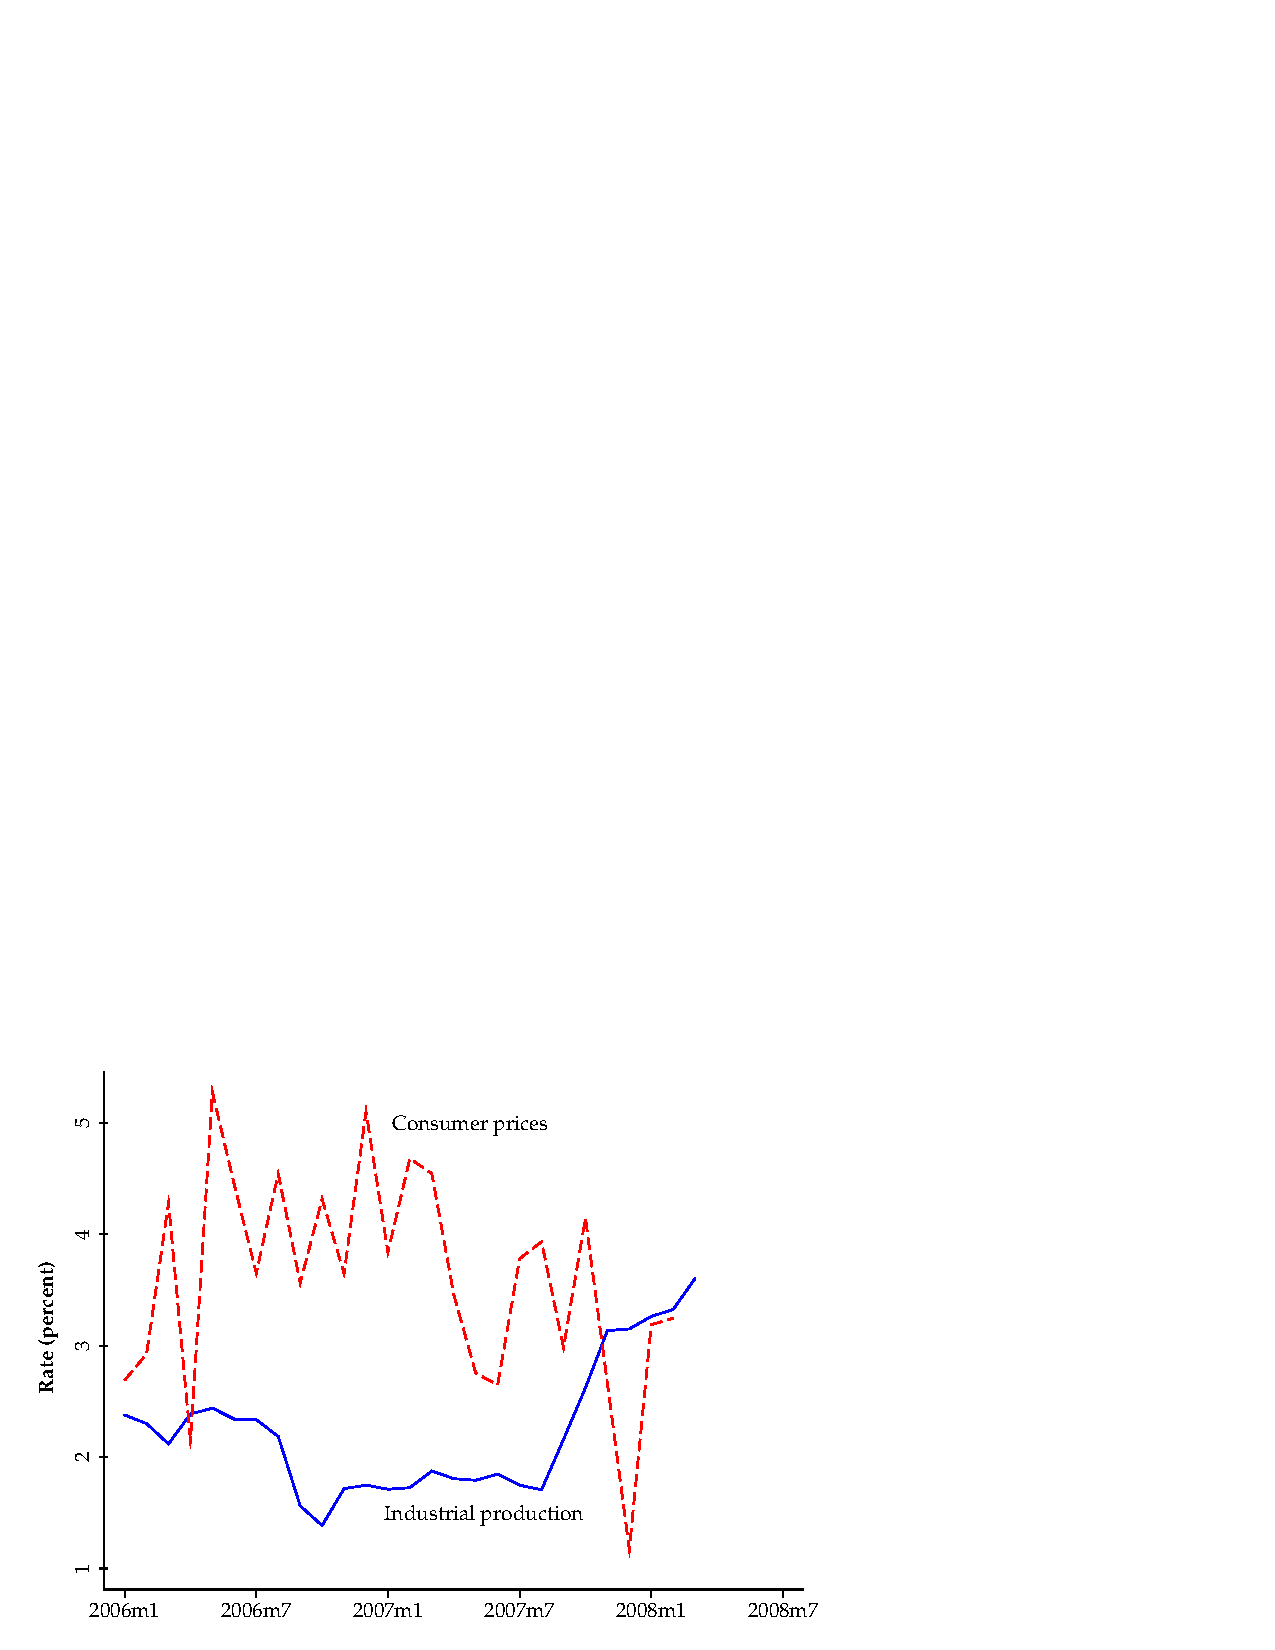
\includegraphics[width=0.8\textwidth]{Figures/eu_asad.pdf}
%    \caption{Growth in prices and industrial production in the
%    Euro Zone.}
%    \label{fig:ez}
%\end{figure}
%
%\item aggregate supply (AS) \index{aggregate supply (AS)}
% and demand in the Euro Zone,
%May 2008.
%As the CFO of Heineken International, you are considering
%the likely evolution of interest rates in the Euro Zone.
%You quickly run through the following questions:
%%
%\begin{enumerate}
%
%\item Over the 2-year period as a whole,
%    what has happened to inflation and output?
%    See Figure \ref{fig:ez}.
%
%\item In the aggregate supply (AS) \index{aggregate supply (AS)}
 and demand framework,
%    do you think the movements in prices and output
%    you mentioned above suggest a shift in supply or demand?  Why?
%    In principle,
%    how should the European central bank \index{central bank} respond to such a shift?
%
%\item How do you think the European central bank \index{central bank} is
%likely to respond?
%How do you see short-term Euro Zone
%interest rates moving over the next 12 months? Why?
%
%\end{enumerate}
%
%
%%\begin{comment}
%Answer.
%\begin{enumerate}
%\item Inflation is up sharply, output is flat to down.
%
%\item The combination in (a) suggests a shift up/left in supply.
%Why?  Because output and inflation have moved in opposite directions.
%Since supply shocks should be accommodated/reinforced,
%the ECB should raise the short-term interest rate.
%
%\item The ECB's primary mission is stable prices,
%so you should see an increase in interest rates.
%This could also be expressed in terms of a Taylor rule,
%possibly with a larger coefficient on inflation
%than output growth.
%\end{enumerate}
\end{enumerate}
\setlength{\leftmargini}{\oldleftmargini}

\section*{If you're looking for more}

The measurement of potential output has generated some interesting debate.
The bottom line, in our view, is that there's usually some question
where the   long-run aggregate supply \index{aggregate supply (AS)!long-run aggregate supply}\index{aggregate supply (AS)}
 curve is. Here is a range of opinion on the subject:
%
\begin{itemize}
\item The Congressional Budget Office (CBO) reviews a number of approaches.
Search: ``cbo potential output.''
%\url{http://www.cbo.gov/sites/default/files/cbofiles/ftpdocs/51xx/doc5191/03-16-gdp.pdf}.

\item Former Fed Governor Frederic Mishkin's speech,
``Estimating potential output,'' is another good overview.
Search:  ``mishkin potential output.''

\item The Kansas City Fed's 2005 Jackson Hole Symposium has
an interesting exchange between Robert Hall and Greg Mankiw.
Hall argues that potential output may very well not be smooth,
which would contradict most measures of it.
As a practical matter, this would change our view of monetary policy dramatically
since many of the movements we see in GDP would be the result of the invisible hand
and, therefore, not something for policymakers to resist.
Mankiw says maybe, maybe not.
Search:  ``Jackson Hole Symposium 2005.''
%\centerline{\url{http://www.kc.frb.org/publications/research/escp/escp-2005.cfm}}
\end{itemize}

\needspace{18\baselineskip}
\section*{Symbols and data used in this chapter}

\begin{table}[H]
\centering
\caption{Symbol table.}
\begin{tabular*}{0.7\textwidth}{l@{\extracolsep{\fill}}l}
\toprule
Symbol & Definition\\
\midrule
$Y$    &Real output (=real GDP)\\
$Y^*$    &Equilibrium (or potential) output\\
${Y^{*}}'$    &New equilibrium (or potential) output\\
AS    &Short-run aggregate supply \\
AS$^*$    &  Long-run aggregate supply\\
AD    &Aggregate demand\\
AD$'$    &Aggregate demand after a shock\\
AS$'$    &Aggregate supply  after a shock\\
\bottomrule
\end{tabular*}
\end{table}

\begin{table}[h]
\centering
\caption{Data table.}
\begin{tabular*}{0.7\textwidth}{l@{\extracolsep{\fill}}l}
\toprule
Variable & Source\\
\midrule
NBER recession indicator    &USRECM\\
CBO real potential GDP        &GDPPOT\\
Oil Price (WTI)                &OILPRICE\\
\bottomrule
\addlinespace
\end{tabular*}
\begin{minipage}{0.7\textwidth}
\footnotesize{To retrieve the data online, add the identifier from the source column to \url{http://research.stlouisfed.org/fred2/series/}.
For example, to retrieve oil prices, point your browser to
\url{http://research.stlouisfed.org/fred2/series/OILPRICE}}
\end{minipage}
\end{table}
